% %%%%%%%%%%%%%%%%%%%%%%%%%%%%%%%%%%%%%%%%%%%%%%%%%%%%%%%%%%%%%%%%%%%%%%%%%%%%
\chapter{Background}%
\label{chap:background}
% %%%%%%%%%%%%%%%%%%%%%%%%%%%%%%%%%%%%%%%%%%%%%%%%%%%%%%%%%%%%%%%%%%%%%%%%%%%%
\section{Key concepts}
\label{backgound:basics}
In this chapter, we first introduce some key concepts necessary for understanding this work and establish common ground.
Some of the concepts are well-known in the community, however, we still consider it suitable to mention them here and provide the reader with references to literature for detailed descriptions.

\subsection{Dialogue System implementations}
\begin{table*}[t]
\small
\setlength\fboxsep{2pt}
        \centering
        \begin{tabular}{rll}
        \textbf{\texttt{USER:}} & \textit{\texttt{I would like a cheap restaurant.}} & \textbf{\texttt{\colorbox{pastelyellow}{inform}(\colorbox{lightblue}{price}=\colorbox{pastelgreen}{cheap})}} \\
        \textbf{\texttt{SYSTEM:}} & \textit{\texttt{Golden plate is cheap.}} & \textbf{\texttt{\colorbox{pastelyellow}{inform}(\colorbox{lightblue}{name}=\colorbox{pastelgreen}{Golden plate})}} \\
        \hdashline[1.5pt/2pt]
        \textbf{\texttt{USER:}} & \textit{\texttt{What is the cuisine?}} & \textbf{\texttt{\colorbox{pastelyellow}{request}(\colorbox{lightblue}{cuisine})}} \\
        \textbf{\texttt{SYSTEM:}} & \textit{\texttt{They serve chinese food.}} & \textbf{\texttt{\colorbox{pastelyellow}{inform}(\colorbox{lightblue}{cuisine}=\colorbox{pastelgreen}{chinese})}} \\
        \hdashline[1.5pt/2pt]
        \textbf{\texttt{USER:}} & \textit{\texttt{Sounds good. Bye!}} & \textbf{\texttt{\colorbox{pastelyellow}{goodbye}()}} \\
        \textbf{\texttt{SYSTEM:}} & \textit{\texttt{Have a great day.}} & \textbf{\texttt{\colorbox{pastelyellow}{goodbye}()}} \\
        \end{tabular}
\normalsize
        \caption{Example of task-oriented dialogue in the restaurant reservation domain. Utterance representations as dialogue acts are depicted on the right. Intents are highlighted in orange, slot names in blue and respective values in green. Note that not all dialogue acts include slots and values}
    \label{fig:das}
\end{table*}
First we describe various approaches to the construction of dialogue systems pipelines and provide some insights about approaches to modeling of the underlying processes.
Because of the varying use cases of Dialogue Systems (DS), the architectures may vary a lot.
We thus introduce a classification of dialogue systems that reflects the expected capabilities.
There are multiple approaches to defining a dialogue system taxonomy in the literature.
Here we introduce the widely used classification scheme \cite{jurafsky2000speech}.
\begin{enumerate}
    \item \textbf{Question Answering (QA)} - Although sometimes not mentioned in the context of dialogue systems, QA task can be seen as an instance of a simple conversation. The main task of a QA system is to provide answers to the user's questions.
    The topics may vary a lot and good understanding is essential for this task as well as knowledge representation.
    The dialogues are usually quite simple and often consist of just one question and the respective answer.
    \item \textbf{Task-oriented DS} - In this setting, the system's goal is to complete a task based on the user's instructions.
    The successful completion may depend on several attributes that the system has to learn from the user utterances.
    The system is also allowed to ask for additional information if needed and typically works with some external source of information such as a database.
    Here the dialogues are usually much more complex than in the QA setting and dialogue context has to be taken into account.
    \item \textbf{Chit-chat} - In some cases, we might be interested in a system that is able to talk to the user casually and provide entertainment.
    Such systems might be used in combination with task-oriented systems to serve as human-like virtual assistants or possibly use the dialogue to advertise products etc.
    The context and knowledge base are also important, but in most cases, there is no well-defined task to be completed, so the evaluation is subjective.
\end{enumerate}

Another way of classifying the dialogues considers their domain of operation.
\textbf{Single-domain} systems are able to work only in one topic area, e.g. public transport or restaurant information, whereas \textbf{multi-domain} systems are able to handle multiple domains.
These types of systems aren't able to give meaningful answers outside of the domains that they're trained on.
A dialogue system is considered \textbf{open-domain} if it's able to have a conversation not limited to a predefined set of domains.
In practice, this is achievable only to some extent since the knowledge base of the program is always limited.
However, with internet access and smart information retrieval methods, the systems are able to cover tens of different domains.

Here we focus on the task-oriented DS and discuss it in more depth.
From the domain perspective, task-oriented DS are usually either single or multi-domain systems, open-domain is not often the case, at least in the research community.
We can see a task-oriented dialogue as a slot-filling task.
That means we have a predefined set of semantic \textit{slots} that need to be filled with the right \textit{values}.
Each utterance in the task-oriented dialogue is considered an action that potentially changes the state of the conversation.
Such actions can be represented using \textit{Dialogue Acts (DA)}\cite{core1997coding}.
DA is a tuple consisting of user \textit{intent} (overall meaning of the sentence) and optionally also \textit{slot} and the corresponding \textit{value}.
In case multiple slot values are present, all are considered to have the same intent.
An example dialogue with respective DA representation is depicted in Table \ref{fig:das}.
Most dialogue system modules for limited domains can be implemented by designing a set of rules and templates.
Such systems can yield satisfying results in some use cases, nevertheless, they are inflexible and generally not considered promising from the research point of view.

\subsubsection{Dialogue System Architectures}
\begin{figure}[t]
    \centering
    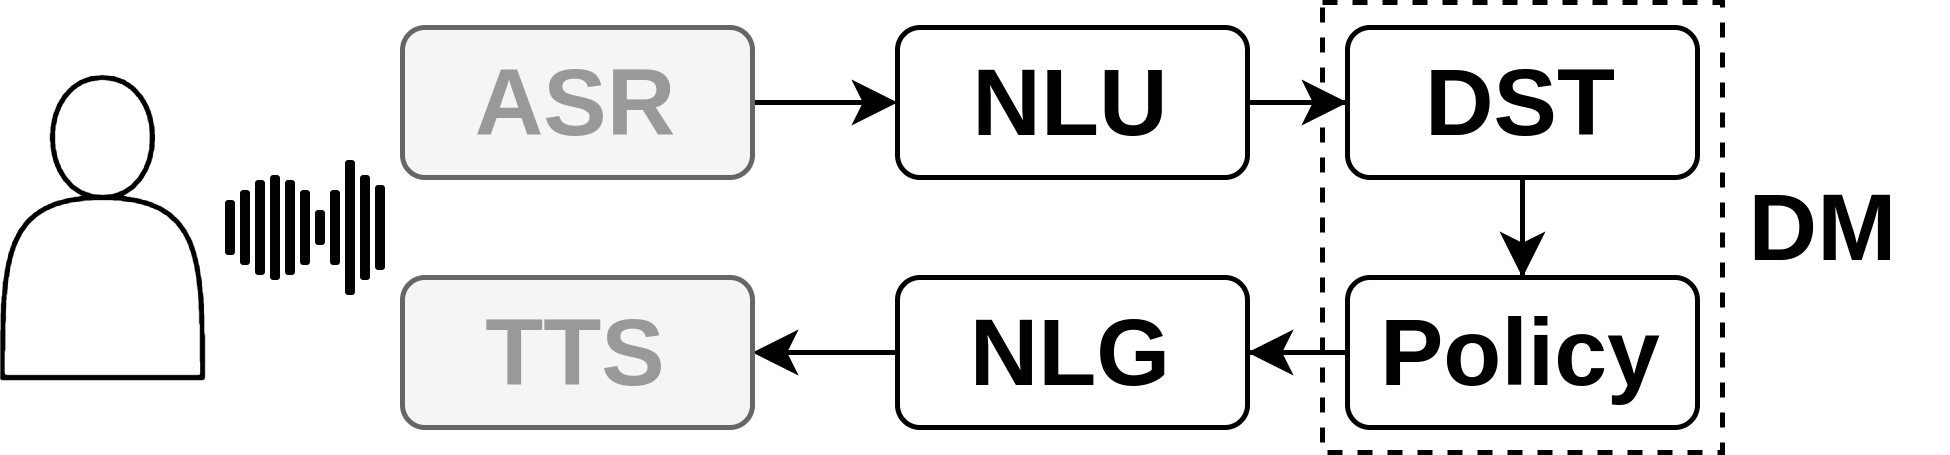
\includegraphics[width=0.80\textwidth]{images/pipeline.png}
    \caption{Overall architecture of task-oriented dialogue system pipeline. The data flow is outlined with arrows. ASR and TTS modules (depicted in gray) are not discussed in this work but are often included with the rest of the components.}
    \label{fig:overall}
\end{figure}
A typical approach to task-oriented DS implementation is to create a modular system with several modules that together handle the conversation flow.
An example of such architecture is depicted in Figure \ref{fig:overall}
We shortly discuss the responsibilities of each component:
\begin{itemize}
    \item \textbf{Natural Language Understanding (NLU)} The purpose of NLU is to extract the meaning of input utterances in natural language and transform it into a structured representation, i.e. dialogue acts.
    Basically, the NLU module has three subtasks.
    It has to determine the domain of the utterance, detect the user intent and capture any slot values, if present.
    \item \textbf{Dialogue State Tracking (DST)} Dialogue state is used to keep track of the dialogue history, effectively providing the necessary context.
    Dialogue State Trackers are used to update the state with correct values after each turn.
    \item \textbf{Dialogue Policy} The core component of the DS is the dialogue policy.
    Its responsibility is to make the decision on which action should the system take at each turn.
    In other words. the responsibility of Dialogue Policy is to guide the dialogue to follow the desired path.
    Dialogue policy together with the DST component are sometimes called \emph{Dialogue Manager}.
    \item \textbf{Natural Language Generation (NLG)} When the decision on a system action is made, the system needs to verbalize the action.
    In other words, we need to create an utterance in natural language that expresses the information given in the system's underlying representation.
\end{itemize}

The module-based approach is advantageous thanks to its good level of explainability.
In case of low performance, we can track the respective modules' outputs and find the source of problems.
On the other hand, error accumulation makes it difficult to recover from errors that were made by the modules early on in the pipeline.
Another disadvantage is the way how these systems are trained.
Each component requires specific data annotation, thus it can be difficult and costly to obtain a dataset suitable for training all of the components.
Also, the system design itself is more complicated since it requires the implementation of multiple models.
Because of the aforementioned drawbacks, a lot of current research works focusing on dialogue modeling end-to-end i.e. using systems that do not consist of explicit components or are able to be trained jointly.

\subsection{Recurrent Neural Networks (RNNs)}
Recurrent Neural Networks are a type of neural network that is well-suited for processing sequential data. Sequential data is data that is ordered in time, such as text or audio.
RNNs are able to learn long-range dependencies between different parts of the input sequence, which makes them well-suited for tasks such as machine translation, text summarization, and question answering.
The motivation for RNNs comes from the fact that human language is sequential by nature and therefore sequential dependencies need to be handled.

The characteristic feature of an RNN is a recurrent connection incorporated into the architecture.
This means that the output of the network at a given time step is fed back into the network at the next time step. This allows the network to encode some information and pass it for future processing, effectively allowing for a concept of memory.

Formally, basic RNN consists of 3 weight matrices: $W_{i}$ to process the input, $W_h$ to process the hidden state, and $W_o$ to construct output.
The computation of output sequence $\mathbf{y} = \{y_0, ..., y_n\}$ from an input sequence $\mathbf{x} = \{x_0, ..., x_n\}$ proceeds in the following steps:
\begin{enumerate}
    \item An initial hidden state $h_0$ is constructed
    \item For time step $t$, first hidden state $h_t$ is obtained using the formula $h_t = f(W_hh_{t-1} + W_ix_t)$. Then, the output is computed as $y_t = W_oh_t$
\end{enumerate}
Note, that the output sequence has the same length as the input sequence which is useful for sequence tagging problems.
However, RNNs can also be used for sequence classification in which case only the last hidden state is considered or the encoder-decoder setup can be used in which one network is used to encode the sequence and second one is used to generate the output which can therefore be of different length.

\paragraph{RNN improvements}
Vanilla RNNs are difficult to train and often fail to memorize long-term dependencies correctly.
Therefore, several extensions were proposed such as LSTM \cite{hochreiter1997} or GRU \cite{cho-etal-2014-properties}
These more complex types of RNNs are able to learn long-range dependencies more effectively.
LSTM and GRU cells have a number of gates that control how information flows through the cell.
These gates allow the RNN cell to learn how to forget irrelevant information and how to remember important parts of the input.
To further improve modeling capabilities, NLP models often employ \emph{bidirectional} RNNs allowing for processing both left and right context.

\paragraph{Training RNNs}
RNNs are trained using a technique called Backpropagation Through Time \cite{werbos1990backpropagation}.
Backpropagation Through Time is a method for training neural networks that deal with sequential data.
The basic idea is to break the sequence into a number of time steps, and then to train the network on each time step individually.

\paragraph{Encoder-Decoder RNNs with attention}
The encoder-decoder RNN is very useful for text-generation tasks like summarization or machine translation.
However, it's very difficult to train RNN on longer sequences, therefore improvements were proposed \cite{bahdanau2014neural,luong-etal-2015-effective} that allow the decoder network to attend to the input sequence and therefore bypass the need to memorize all the information in the hidden state.

\subsection{Transformer}
The Transformer architecture is another neural network architecture capable of processing sequential data.
It was first proposed in \citet{vaswani2017attention}.
Unlike RNNs, the Transformer architecture doesn't work with a hidden state that is being passed forward in time.
Instead, the architecture is based solely on the attention mechanism, which allows the model to learn long-range dependencies between different parts of the input sequence.

The attention mechanism works by allowing the model to focus on different parts of the input sequence when producing the output sequence.
For example, if the model is translating a sentence from English to German, the attention mechanism can allow the model to focus on the English words that are most relevant to the German words that need to be produced.

The original Transformer architecture is composed of an encoder and a decoder.
The encoder takes the input sequence and produces a sequence of hidden representations.
The decoder then takes these hidden representations and produces the output sequence.
The attention mechanism is used at both the encoder and decoder to allow the model to use different parts of the input sequence when producing the output sequence.
The decoding process might be performed both as autoregressive or non-autoregressive, depending on the use case.

Both the encoder and decoder are basically a stack of self-attention layers.
Each self-attention layer takes the hidden representations from the previous layer and produces a new set of hidden representations.

The decoder also includes an attention component that allows the model to attend to the output sequence generated so far when producing the next token.
This allows the model to learn how to generate the output sequence in a way that is consistent both with the input sequence and the prefix generated so far.

The Transformer architecture has been shown to achieve state-of-the-art results on a variety of natural language processing tasks. 
Moreover, the Transformer architecture was used as a base for many models pretrained on large natural language corpora, allowing efficient transfer of the learned information to downstream tasks and thus revolutionizing the NLP field.

\section{Pretrained Language Models (PLMs)}
\label{background:plms}
The appearance of PLMs marked a new era in NLP.
Although Language Modeling with neural networks has been in the community focus for some time with transforming works such as  \citet{mikolov2010recurrent,mikolov2013distributed} it wasn't until ELMo \cite{peters-etal-2018-deep} and ULMFiT \cite{howard-ruder-2018-universal}that we were able to create PLMs that could be finetuned for a variety of tasks with comparably low data requirements.

Shortly after ELMo, models based on the Transformer architecture started to appear such as BERT for efficient language encoding \cite{devlin2019} or GPT for generation \cite{radford2018improving}.
BERT introduced a novel approach to Transformer usage by employing only the encoder part of the original Transformer architecture.
Importantly, BERT pretraining introduced the task of Masked Language Modeling, randomly masking some of the input tokens and reconstructing them correctly at the output.
Additionally, BERT is trained to estimate the probability that two input sentences follow each other.
These pretraining techniques make BERT great at encoding natural language inputs into useful representations.
GPT on the other hand consists only of Transformer decoder blocks.
It is trained for next token prediction, so it is capable of autoregressive Language Modeling.
Therefore GPT is a perfect candidate for a base model to be finetuned on language generation tasks including machine translation, summarization etc.


Both BERT and GPT showed great potential for finetuning on downstream tasks and established themselves as strong baselines for many NLP tasks and benchmarks.
They are often referred to as \emph{foundational} models because of their abilities of language understanding and generation and the potential to apply these abilities to various tasks.
From a certain point of view, the usability of PLMs lies in the fact that they are able to create useful and contextual representations of input words and phrases, often called \emph{(word) embeddings}.
This ability has been observed in the word2vec model \cite{mikolov2013distributed} and improved by ELMo \cite{peters-etal-2018-deep}, BERT \cite{devlin2019}, SBERT \cite{reimers2019sentence} and others.

Many model architectures based on Transformer blocks followed both for encoders \cite{liu2019roberta,reimers2019sentence}; decoders \cite{radford2019language,brown2020language} or even sequence-to-sequence \cite{raffel2020exploring,lewis-etal-2020-bart}.
These models were largely adopted by the NLP community.


\subsection{Large Language Models (LLMs)}
The foundational models changed the NLP paradigm but still need substantial in-domain data in order to achieve good performance on some tasks.
Moreover, finetuning those larger models requires more computational resources, therefore more lightweight methods to adapt the models to downstream tasks were proposed s.a. Transformer Adapters \cite{pfeiffer2020AdapterHub}.
However, as researchers started to scale up the models with GPT-2 and GPT-3 leading the efforts \cite{radford2019language,brown2020language}, new abilities started to emerge \cite{wei2022emergent}.
With model sizes exceeding billions of parameters, the large pre-trained Transformer decoders are able to perform many tasks that they weren't explicitly trained for \cite{brown2020language}.
Such large models are capable of performing tasks like summarization, translation, question answering, or even reasoning and arithmetics to some extent without any task-specific training.
Those tasks can be presented to the LLMs purely in the form of textual task descriptions in the inference time.
This approach of \emph{in-context learning} is frequently used with great success \cite{min2022rethinking,dong2022survey}.
The textual input for LLMs is frequently referred to as a \emph{prompt}.

\paragraph{On LM scaling}
Scaling laws in language models describe the relationship between the size of a language model and its performance.
It has been shown, that with the next token prediction objective (which is what virtually all LMs are trained for) some abilities start to emerge when exceeding a certain size threshold \cite{kaplan2020scaling}.
However, bigger models also need to be trained longer and with more data \cite{hoffmann2022training}
In general, larger language models tend to perform better than smaller models, but they also require more computational resources to train.
This line of research can help us understand how the size of a language model affects its performance and to predict the performance of a language model before it is trained.

\paragraph{Instruction Tuning}
Although the LLMs have great abilities and potential to accomplish a variety of different tasks, it is not always straightforward to provide them with correct instructions.
Therefore significant effort was made to \emph{align} the LLMs better with the human requirements.
Consequently, even rather inexperienced users can instruct the model to accomplish custom tasks according to their needs.
For this purpose, reinforcement learning techniques were explored \cite{ziegler2019fine,ouyang2022training}.
Although these techniques proved to be quite effective, the process is still very demanding in terms of collecting feedback from users.
Consequently, several datasets were proposed \cite{supernaturalinstructions,black2022gpt} that contain tasks like summarization, reasoning, etc. formulated using instructions in natural language and desired outputs.
These datasets allow tuning the models either using reinforcement learning or supervised finetuning methods.

\paragraph{Prompt engineering vs. LLM finetuning}
The in-context learning approach has great advantages because it makes it possible to obtain great performance from LLMs by simply formulating the task and desired output structure in the LLM input (i.e. prompt).
Although this approach might be very efficient for some tasks, especially those that are well described in the corpora available to the LLM during training \cite{wei2022emergent}, some more specific tasks might yield better results after finetuning of the model \cite{tu-etal-2022-prompt}.
However, the LLM finetuning process is quite demanding in terms of computational resources, therefore alternative approaches were proposed s.a. LoRA \cite{hu2021lora} or Transformer Adapters \cite{pfeiffer2020AdapterHub}.

\section{Variational autoencoders}
\label{background:vae}
\begin{figure}[t]
    \centering
    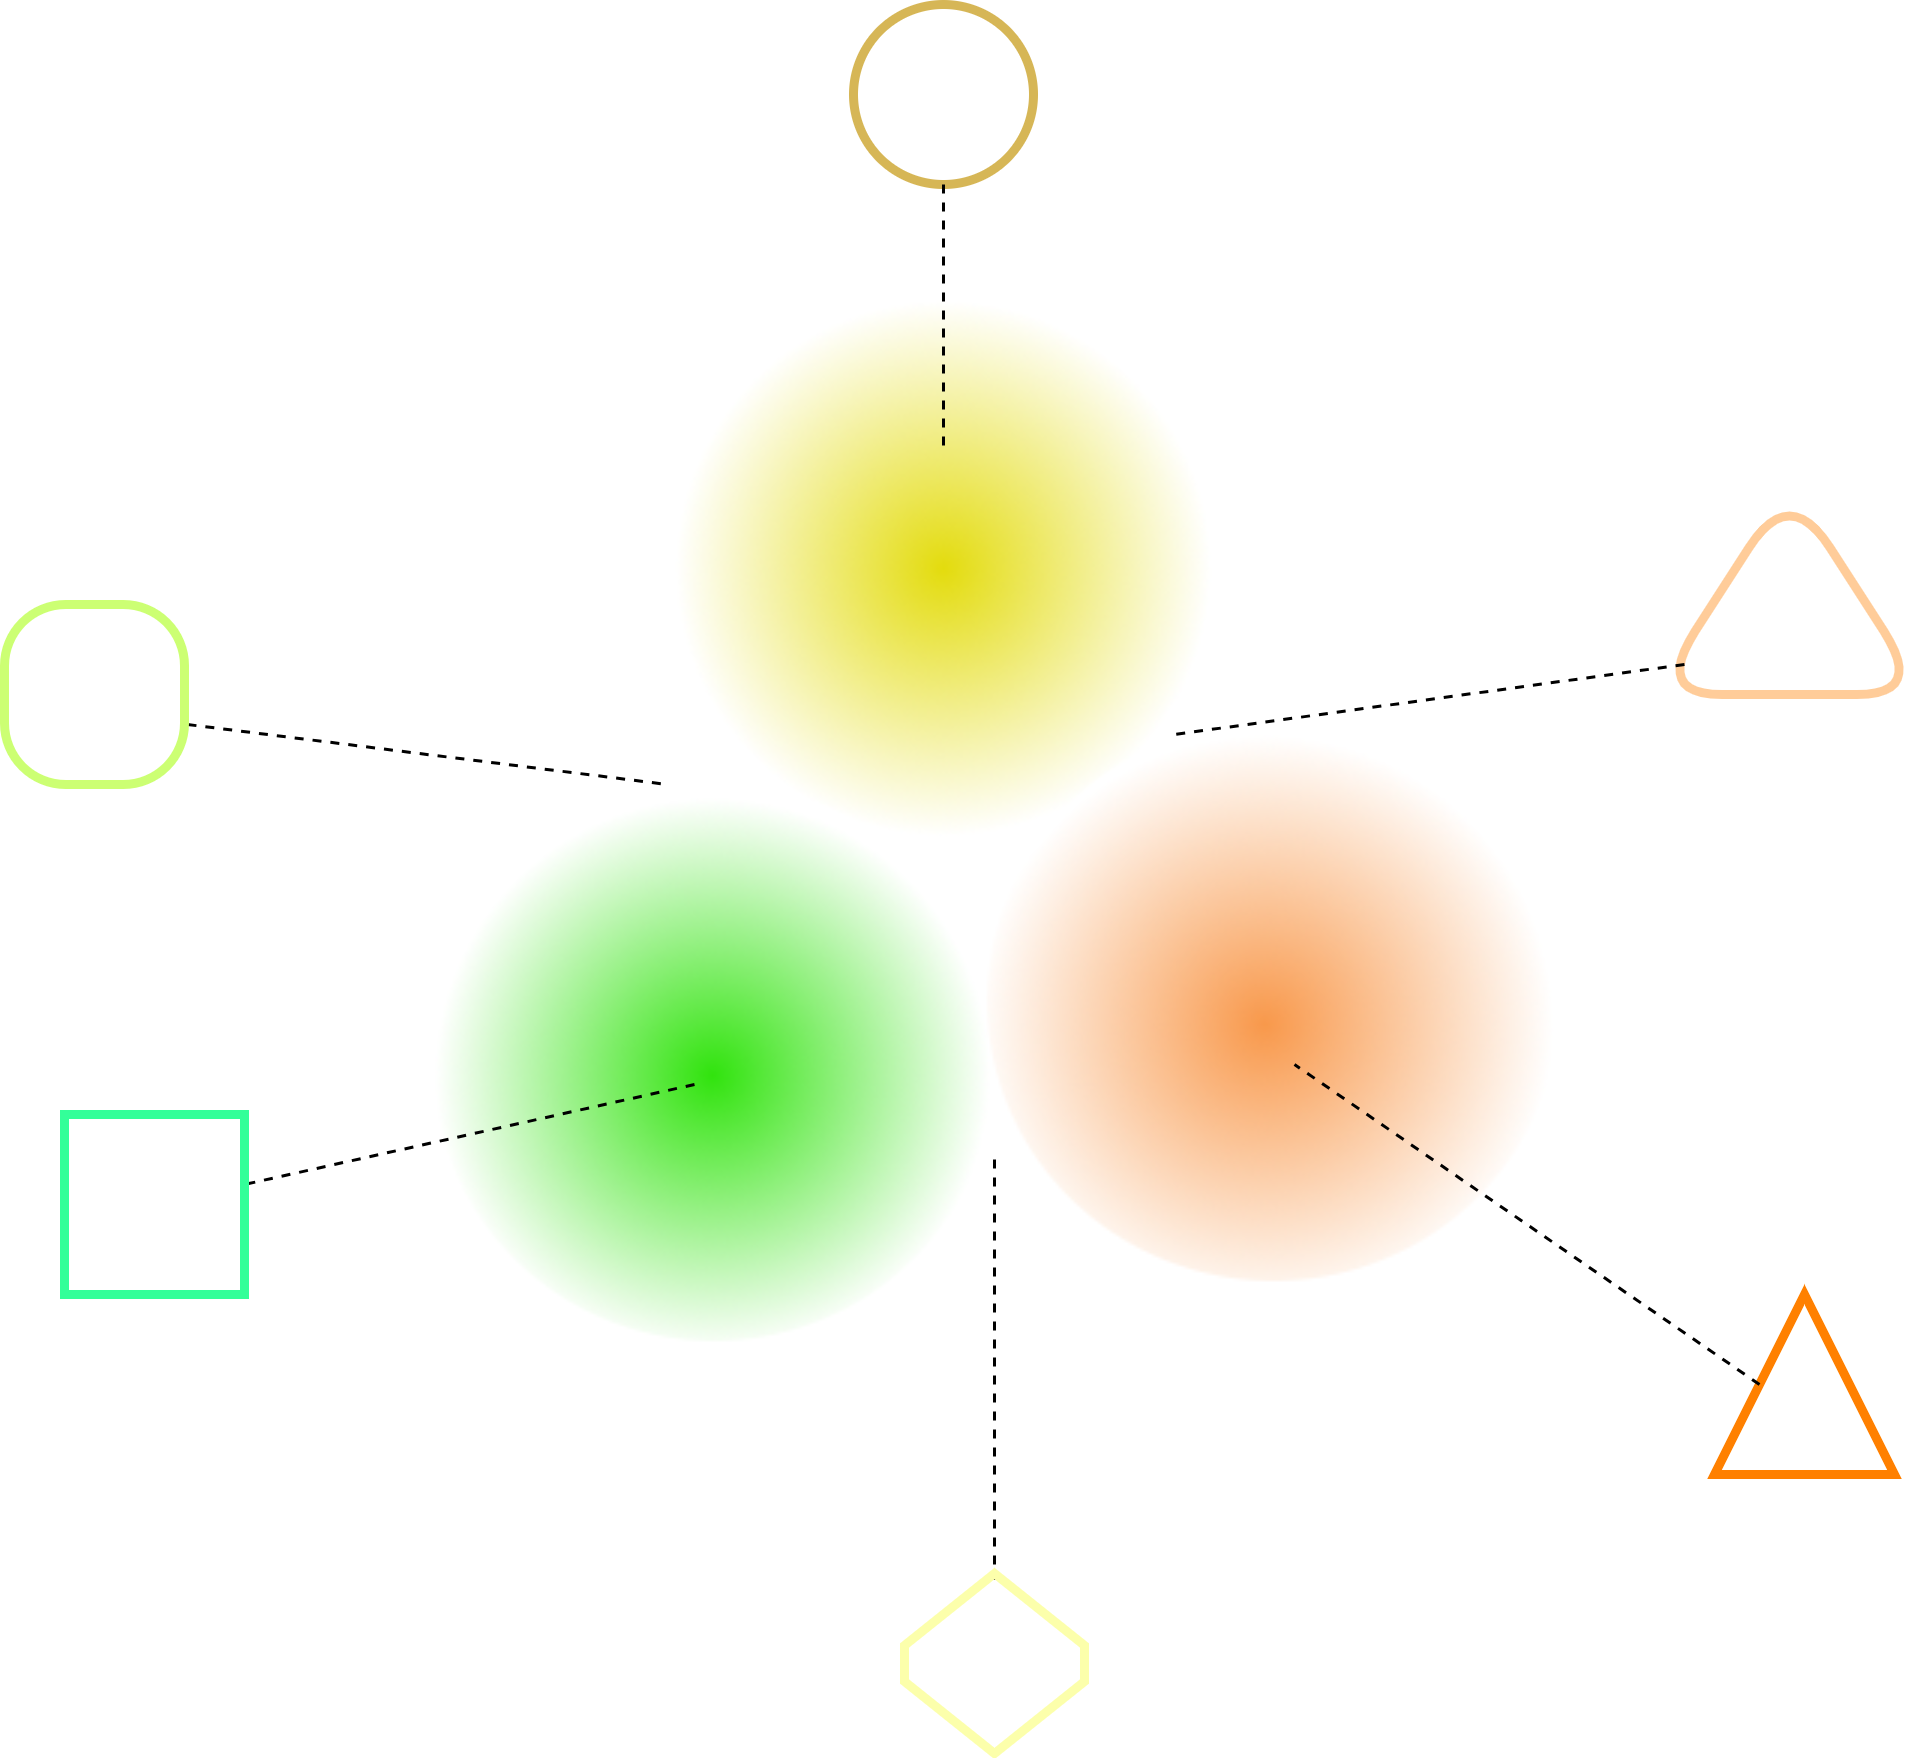
\includegraphics[width=0.46\textwidth]{images/VAE.png}
    \caption{Variational autoencoder latent space. The encoder distributions are distinguished by colors and different classes by shapes. It can be seen, the interpolation between two sampled points is meaningful}
    \label{fig:vae}
\end{figure}
Neural network training is a process during which the network learns to create internal representations of data in order to accomplish a given task.
In case of autoencoders, the task is to encode an input $\mathbf{x}$ in a way that allows for its reconstruction into the original form.
The autoencoder model consists of an encoder function $\varphi^{enc}$, which encodes an input $\mathbf{x}$ into a latent representation $\mathbf{z}$, and a decoder $\varphi^{dec}$, which models the conditional re-generation probability $p(\mathbf{x}|\mathbf{z})$.
In case of sequence autoencoders, both the encoder and decoder can be realized with an RNN.
However, vanilla autoencoders often fail to extract global semantic features of natural language sequences \cite{bowman2015generating}; therefore, adjustments need to be made in order to obtain better representations.
The technique proposed by \citet{kingma2013auto} uses the Variational Autoencoder (VAE) framework to tackle this issue.
The architecture is modified so that $\varphi^{enc}$ represents a recognition model $q(\mathbf{z}|\mathbf{x})$ which parameterizes an approximate posterior distribution over $\mathbf{z}$.
VAEs impose prior distribution on the latent variable $\mathbf{z}$, which acts as regularization during training and makes it possible to draw samples from $q$.
Consequently, the VAE latent space is regular in the sense that it is possible to interpolate between two points and obtain reasonable representations.
The latent space structure is depicted schematically in Figure \ref{fig:vae}.
Typically, the modeled distributions are Gaussian and the prior is the standard normal distribution $N(0, 1)$.

We can realize the function modules in VAE using neural networks, however, there is a drawback regarding the implementation of sampling.
The sampling operation is not differentiable and therefore cannot be trained using standard approaches.
A solution to this problem is to use the \textit{reparameterization trick} \cite{kingma2013auto}.
The reparameterization trick exploitsexploitsexploitsexploits the fact that a random variable under certain conditional distribution can be expressed as a deterministic transformation of some other variable with independent marginal distribution.
Distributions that allow us to do such a transformation include \textit{Gaussian, Logistic} or \textit{Gumbel}.

\subsection{VAE latent space discretization}
\label{background:vae_discrete}
Although VAE training yields robust representations that are also more interpretable thanks to the regularized latent space, in some cases, we require the latent representations to be discrete.
The motivation is mainly to improve interpretability and possibly uncover underlying processes in sequential tasks.
It is problematic to incorporate discrete variables into neural network models, because the widely used backpropagation algorithm requires smooth differentiable functions in order to propagate the gradients correctly.
\citet{van2017neural} propose a vector quantization technique to discretize the latent variables in VAEs.
Another approach is to use the Gumbel-softmax distribution \cite{jang2016categorical} that enables together with the reparameterization trick (Section \ref{04:to-unsup}) to work with categorical variables while not breaking the gradient flow in the network.

\subsection{Variational Recurrent Neural Networks}
\label{background:vrnn}
The VRNN model \cite{chung2015recurrent} can be seen intuitively as a recurrent network with a VAE in every timestep.
It extends the VAE model to a sequence of observations generated from a series of hidden latent variables $\mathbf{z}$.
Formally, we want to estimate the joint probability distribution of a sequence of observed and corresponding latent variables $p(\mathbf{x}, \mathbf{z}) = p(\mathbf{x}|\mathbf{z})p(\mathbf{z})$.
The conditional distribution $p(\mathbf{x}|\mathbf{z})$ is parameterized with a neural network.
However, we still need to estimate the posterior $p(\mathbf{z}|\mathbf{x})$ in order to connect the latent variables with the observations.
The VAE uses a variational approximation $q(\mathbf{z}|\mathbf{x})$ that allows maximizing the lower bound of the log-likelihood of the data:
\begin{equation}
\begin{split}
    \log~p(\mathbf{x}) \ge -\mathrm{KL}(q(\mathbf{z}|\mathbf{x})||p(\mathbf{z}))\\ + \mathbb{E}_{q(\mathbf{z}|\mathbf{x})}[\log~p(\mathbf{x}|\mathbf{z})]
    \label{eq:vae}
\end{split}
\end{equation}
where KL is the Kullback-Leibler divergence.
We consider a prior  network $\varphi_{prior}$ and a posterior network $\varphi_{post}$, which compute the parameters of $p(\mathbf{z})$ and $q(\mathbf{z}|\mathbf{x})$ respectively.
In a VRNN, $\varphi_{prior}$ and $\varphi_{post}$ additionally depend on the RNN hidden state $\mathbf{h}^t$ to allow for a context-aware prior distribution.
In each time step, we obtain the distribution parameters as follows:
\begin{equation}
\label{eq:distr_theta}
\begin{gathered}
    \mathbf{\theta}_{q}~=~\varphi_{post}(\mathbf{h}^t, \varphi_{enc}(\mathbf{x}^t))\\
    \mathbf{\theta}_{p}~=~\varphi_{prior}(\mathbf{h}^t)
\end{gathered}
\end{equation}
where $\varphi_{enc}$ is the encoder and $\theta_q, \theta_p$ are parameters of the respective distributions (see Section \ref{sec:method_latent}).
With distribution parameters available, we can sample the latent variable and predict the output:
\begin{equation}
\label{eq:x_infer}
\begin{gathered}
    \mathbf{z}^t~\mathtt{\sim}~p(\mathbf{z};\theta_{p})\\
    \mathbf{x}^t~=~ \varphi_{dec}(\mathbf{z}^t)
\end{gathered}
\end{equation}
where $\varphi_{dec}$ represents the decoder network.
The update of the hidden state $\mathbf{h}^t$ is as follows:
\begin{equation}
    \label{eq:hidden_update}
    \begin{gathered}
        \mathbf{h}^{t+1} = \text{RNN}([\varphi_{enc}(\mathbf{x}^t),\varphi_{z}(\mathbf{z}^t)], \mathbf{h}^t)
    \end{gathered}
\end{equation}
where $[.,.]$ is concatenation, $\varphi_z(.)$ is a feature extractor and $\text{RNN}()$ is a step transition function of a recurrent neural network, in our case an LSTM \cite{hochreiter1997}.

\section{Memory Networks}
\label{background:mem_nn}
\begin{figure}[t]
    \centering
    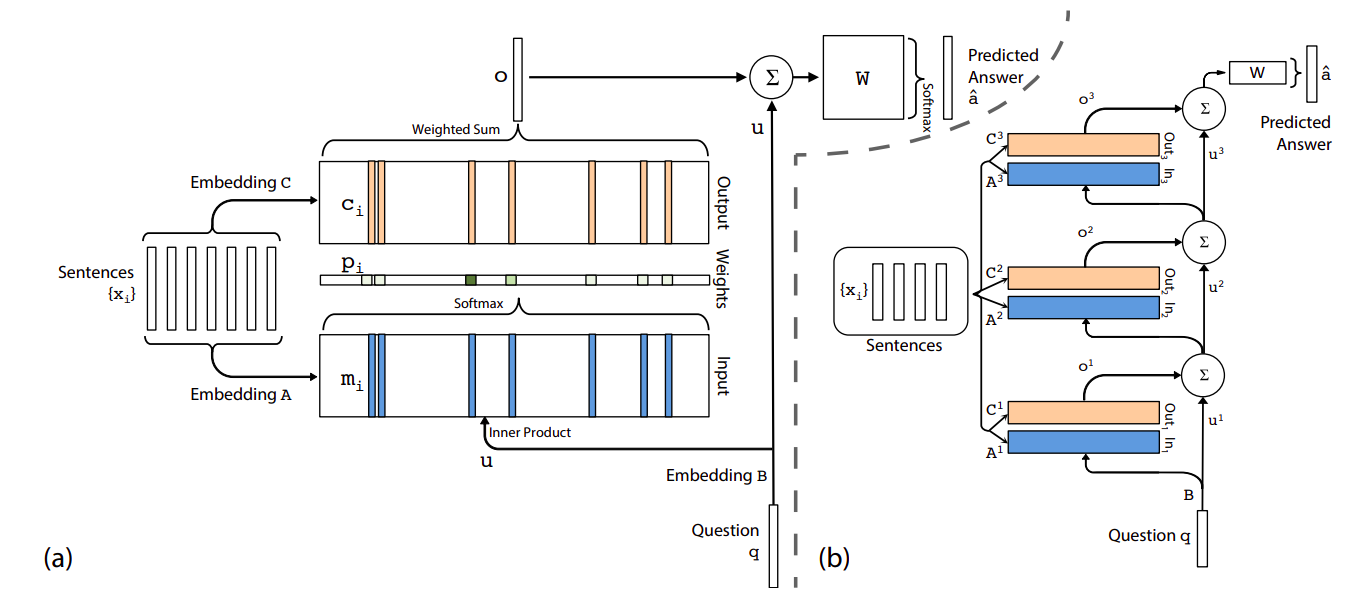
\includegraphics[width=\textwidth]{images/e2e_mem_nn.png}
    \caption{The end-to-end Memory Network model introduced in \citet{sukhbaatar2015end}. It shows the computation process of (a) a single-layer and (b) 3-layer version of the model. }
    \label{fig:e2e_memnn}
\end{figure}
The Memory Network model (MemNN) addresses the issue associated with RNN networks which typically suffer from catastrophic forgetting and exponential decay of stored information \cite{neil2016phased}.
The Memory Network model was originally introduced in \citet{DBLP:journals/corr/WestonCB14}.
\subsection{The Memory Network architecture}
The key idea behind memory networks is to incorporate an external memory component into the network architecture, allowing the model to store and access information over long sequences of inputs.
The memory component acts as a separate storage module, similar to a computer's memory, which the network can read from and write to during its computation.
The MN model architecture's main component is a memory array $\mathbf{m} = \{\mathbf{m}_1,...,\mathbf{m}_n\}$.
The basic Memory Network takes an input $\mathbf{x}$ and processes it in four processing steps:
\begin{enumerate}
    \item The input $x$ is processed with \emph{input feature map} $I$ to obtain internal representations of the input $I(x)$.
    \item The memory array is updated using the \emph{generalization component} $G$. In this step, each memory entry gets update following the equation $\mathbf{m}_i = G(\mathbf{m}_i, I(\mathbf{x}), \mathbf{m})$.
    \item The output features are computed with the \emph{output feature map} using the memory and transformed input $ o = O(I(\mathbf{x}, \mathbf{m})$
    \item Finally, the output representation is used to decode the final response: $r = R(o)$
\end{enumerate}

In general, the components $I, G, O$ and $R$ can be represented with any function capable of doing the task.
However, in most cases in the literature, we see models that use neural networks to instantiate these components.
Consequently, the whole model is end-to-end differentiable and thus trainable with algorithms s.a. backpropagation.
We talk about Memory Neural Networks (MemNNs).
Although various kinds of data can be input and output to MemNNs in general, in this work we consider only MemNNs that work with text.
Let us describe a basic MemNN for text.
When given text input, such a basic model can simply save each text memory into a new memory slot.
Therefore, old memories are not updated and new inputs are stored sequentially.
The most interesting components of this simple text model are $O$ and $R$.
The $O$ module scores the saved memory vectors given text input $x$ and subsequently retrieves $k$ supporting entries with the highest scores from the memory.
To produce a response, the $R$ module takes the input $x$ and $k$ retrieved memories and generates an output either by copying one of the memories or truly generating new outputs, for example with an auto-regressive RNN decoder. 

\subsection{Multi-hop end-to-end MemNN}
The MemNN architecture's disadvantage is that it requires supervision at each layer during training as pointed out by \citet{sukhbaatar2015end}.
In this work, the authors address this problem and present a fully end-to-end trainable memory network model which we call \emph{e2eMemNN}.
In the e2e MemNN, the input takes a set of inputs $x$ to be stored in the memory and a query $q$.
Each input $x_i$ is then embedded with two distinct embedding functions $E_m$ and $E_c$ to obtain a memory entry $m_i$ and corresponding output embedding $c_i$ respectively.
The query $q$ is then embedded as well with the different function $E_q$ to obtain query embedding $u$.

\begin{figure}[t]
    \centering
    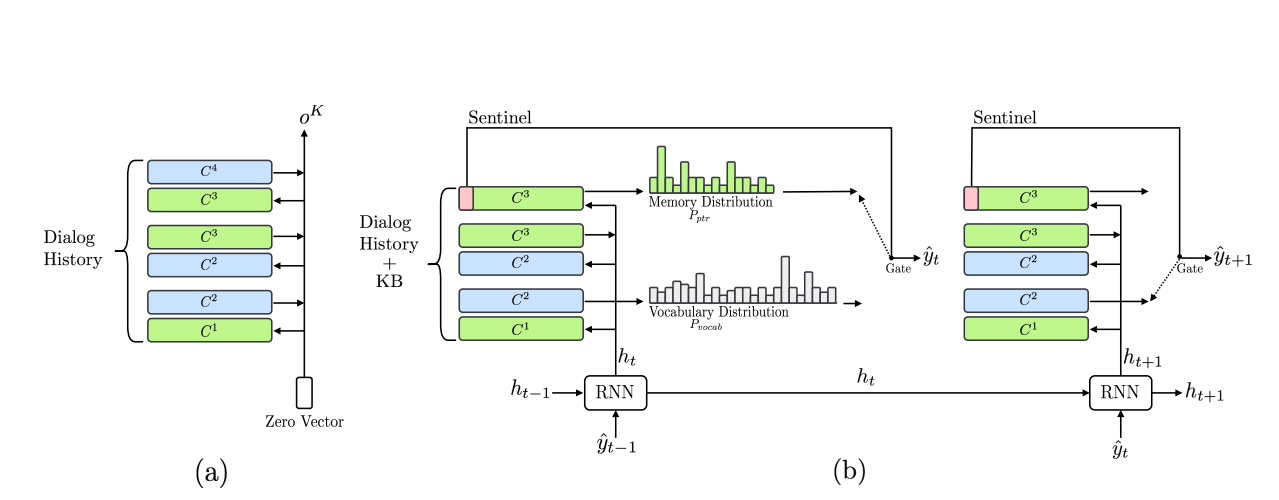
\includegraphics[width=\textwidth]{images/mem2seq.png}
    \caption{The Mem2Seq model \cite{madotto-etal-2018-mem2seq} showing the memory encoder with 3 hops (a) and 2 steps of the memory decoder (b) }
    \label{fig:mem2seq}
\end{figure}

After embedding, a memory distribution $p$ is computed as a match between $u$ and each memory $m_i$ as $softmax (u^Tm_i)$.
The memory distribution $p$ is then used to create an output $o$ computed as a weighted sum over the output embeddings $\sum_i p_ic_i$.
The output $o$ is then used to produce the final answer which can be a categorical label or textual response generated with an auto-regressive model.

The authors also introduce a multi-layer version of this model.
In the multi-layer version, each layer $k$ has distinct embedding matrices $E^k_m$ and $E^k_c$. The output $o_k$ from layer $k$ is used to form input query embedding $u_{k+1}$ to the layer $k+1$: $u_{k+1} = u_k + o_k$.
The multi-layer processing is sometimes also referred to as \emph{multi-hop} where a \emph{hop} refers to processing by one layer.

\subsection{Mem2Seq model}
The Mem2Seq model \cite{madotto-etal-2018-mem2seq} is a task-oriented dialogue model that builds on top of the end-to-end architecture introduced in \citet{sukhbaatar2015end}.
The architecture is described in Figure \ref{fig:mem2seq}.
The model consists of encoder and decoder parts.
The encoder is a 3-hop Memory Network that encodes the dialogue context.
The more interesting part is the decoder which is a Recurrent Neural Network enhanced with Memory Network in every time step.
This Memory Network contains conversation history and knowledge base entries encoded as memory vectors.
At each step, the hidden state of the RNN is used as a query vector. Then a distribution over memory is computed, as described earlier. 
Also, a distribution over vocabulary is computed from the RNN hidden state, similar to standard RNN-based decoders.
One special entry is added to the memory, so-called \emph{sentinel}.
If the highest probability is assigned to the sentinel token, the vocabulary distribution is used to generate the next token.
Otherwise, the next token is chosen according to the memory distribution.
In other words, at each generation step, the model uses the RNN state to decide whether to copy something from the memory (conversation history + knowledge base info) or generate an arbitrary new token from vocabulary distribution.
This way the model is able to effectively use information from the past.

\section{Datasets}
\label{02:sec:input-data-desc}
We provide descriptions of some of the most prominent datasets we use for our experiments.
Most of them are largely used in the dialogue community and provide common benchmarks used for the evaluation.
All these datasets have several task-oriented dialogue properties in common that define the conversation according to \cite{young2013}:
\begin{enumerate}
\item \textbf{Domain(s)} define the topic (or range of topics) which are mentioned in the dialogue. There can be several domains per dialogue.
\item \textbf{Task} -- the users in each of the dialogues are attempting to reach a certain goal (such as booking a restaurant or finding a tourist attraction).
\item \textbf{Turns} We consider \emph{turn-taking} dialogues, i.e.\ the participating sides exchange utterances alternately.
One such utterance exchange is called a dialogue turn.
Utterance itself is considered the linguistic realization of the speaker's thoughts and will. It can be spoken or written. 

The meaning of each utterance can be represented in a structured way with \textbf{Dialog Act(s)} \cite{Weisser2016}.
It is a meta-information that emerges from the respective utterance and qualifies it. It describes the beliefs, desires, and intentions.
Dialogue acts can be represented using \emph{Domains}, \emph{Intents} and \emph{Slots}. The intent represents the user intention, i.e.\ the sub-goal that the user wants to achieve with a particular utterance.
Slots represent the attributes that instantiate the dialogue act.
Each domain is associated with a certain set of intents, and each intent can be combined with multiple slots. A slot, however, can be used by multiple intents as well.
We provide statistics about the dialogue datasets we use in this work in Table \ref{02:tab:data_stats} and some samples in Tables \ref{02:tab:mw_example} and \ref{02:tab:smd_example}.
\end{enumerate} 
\subsection{Datasets description}
\paragraph{MultiWOZ} (MW) is an established task-oriented dataset introduced by \cite{budzianowski-etal-2018-multiwoz}. It's been released in several versions, the standard most commonly used nowadays are MultiWOZ 2.1 and MultiWOZ 2.2.
MultiWOZ 2.2 is an improved version of the original dataset by (1) fixing some annotation errors, inconsistencies, and ontology issues, (2) adding slot span annotations for utterances.
MultiWOZ contains more than 10,000 annotated dialogues and spans several domains.
The data were gathered via a crowd-sourcing Wizard-of-Oz scheme which is described in \cite{wen-etal-2017-wizard-of-oz}.

\paragraph{DSTC2} \cite{henderson_robust_2014} was introduced as a part of a challenge to improve state tracking within dialogue systems. It contains over 3,000 dialogues covering a single domain around restaurant reservations. The dialogue corpus was collected using Amazon Mechanical Turk with a POMDP-based spoken dialogue system. It is the only human-machine dataset in our collection.

\paragraph{CamRest676} (CR) \cite{wen2016network} is another crowd-sourced dialogue corpora gathered via the Wizard-of-Oz scheme. CamRest with its 676 conversations is the smallest of the datasets used in this work, and it is also a single-domain dataset focused on helping users to find a restaurant in Cambridge, UK. 

\paragraph{Schema-guided dialogue} (SGD) is a large (more than 20,000 dialogues) multi-domain (around 20 domains covered) dataset containing in total 45 API services based on a pre-defined schema. First, the data was collected via a simulator that interacts with the API services, and then the dialogues were paraphrased using crowd-sourcing. \\

\paragraph{ATIS} (AT) \cite{hemphill_atis_1990} contains utterances taken from conversations about flight searches and reservations. \footnote{There are multiple ATIS data versions available. We used one from \url{https://www.kaggle.com/siddhadev/atis-dataset-from-ms-cntk}.}
\paragraph{Cambridge SLU} (CS) \cite{henderson2012discriminative} resembles the CamRest 676 dataset but is larger and focuses only other user part of the conversations.

\paragraph{Stanford Multidomain Dialogues} (SMD) \cite{eric-etal-2017-key} contains concise dialogues between a driver and an in-car virtual assistant about appointments, navigation, etc.
The dataset assumes interaction with the database or external APIs, however, the information is provided with each dialogue in the form of relevant Knowledge Base entries.

\begin{table}[t]
    \centering\footnotesize
    \begin{tabular}{l@{\hspace{0.8em}}r@{\hspace{0.3em}}r@{\hspace{0.3em}}r@{\hspace{0.3em}}r@{\hspace{0.3em}}r@{\hspace{0.3em}}r@{\hspace{2em}}r}
        \toprule
        \textbf{Data}         & \textbf{SGD} & \textbf{MW} & \textbf{DSTC} & \textbf{CR} & \textbf{SMD} & \textbf{ATIS} & \textbf{Total} \\ \midrule
        \textbf{Domains}        & 18        &    7        &      1        &      1  & 3 & 1  &    19$^{\ast}$ \\
        \textbf{Slots}        & 145       &    29       &     10        &      7    & 15 &  79 & 166$^{\ast}$ \\
        \textbf{Dialogues$^{\ast\ast}$}       & 22.8    & 10.4     &    3.2     &      0.7    & 3 & -- & 37.1\\
        \textbf{Turns$^{\ast\ast}$}        & 463.3   & 143.0     &    51.0  &     5.5   & 16.1 & 4.9 & 662.8\\
        \textbf{Turns/Dial.}   & 20.30     & 13.71       &   15.77        &     8.12   & 5.25 & -- & 17.83 \\
        \textbf{Avg. utt. length} & 9.86      &  13.23      &   8.47        &  10.71     & 9 & 11.37  & 10.49 \\
        \textbf{Unique Words}$^{\ast\ast}$ & 32.3 & 23.2 & 1.3 & 1.7   & 1.6 & 0.9 & 49.9 \\

     \bottomrule
    \end{tabular}
    \caption{Basic statistics of the datasets we use in this work. Overall and for individual sources (number of domains and slots, total numbers of dialogues and turns, average number of turns per dialogue, and average utterance length in terms of words. $^{\ast}$ is not a sum due to ontology overlap. $^{\ast\ast}$ in thousands.}
    \label{02:tab:data_stats}
\end{table}

\begin{table}[h]
    \centering
    \begin{tabular}{l|l}
    \toprule
         \textbf{User} & \texttt{I need to book a hotel in the {\color{cyan!80!yellow!80!black!100 }east} that has { \color{orange!50!yellow!90!black!100!}4 stars.}} \\
         \textbf{System} & \texttt{I can help you with that. What is your price range?} \\
         \textbf{State} & \texttt{restaurant \{\}, ..., hotel \{"area": "{\color{cyan!80!yellow!80!black!100 }east}", "stars": "{\color{orange!50!yellow!90!black!100!}4}" \}} \\
         \textbf{User} & \texttt{That doesn't matter as long as it has {\color{cyan!80!yellow!80!black!100 }free wifi} and {\color{orange!50!yellow!90!black!100!}parking}.}\\
         \textbf{System} & \texttt{If you'd like something cheap, I recommend the Allenbell.} \\
         \textbf{State} & \texttt{restaurant \{\}, ..., hotel \{"area": "east", "stars": "4",}\\
         & \texttt{"wifi": {\color{cyan!80!yellow!80!black!100}yes}", "parking": "{\color{orange!50!yellow!90!black!100!}yes}"\}} \\
         \bottomrule
    \end{tabular}
    \caption{A simplified example taken from the MultiWOZ corpus}
    \label{02:tab:mw_example}
\end{table}


\begin{table}[h]
    \centering
    \begin{tabular}{l|l}
    \toprule
         \textbf{Driver} & \texttt{What {\color{cyan!80!yellow!80!black!100}gas stations} are here?} \\
         \textbf{NLU} & \texttt{\{"poi\_type": "{\color{cyan!80!yellow!80!black!100}gas stations}" \}} \\
         \textbf{Car} & \texttt{There's a Chevron} \\
         \textbf{Driver} & \texttt{That's good! Please pick the {\color{cyan!80!yellow!80!black!100}quickest} route }\\ & \texttt{to get there and {\color{orange!50!yellow!90!black!100!}avoid all heavy traffic}!} \\
         \textbf{NLU} & \texttt{\{"distance": "{\color{cyan!80!yellow!80!black!100}quickest}",} \\
            & \texttt{"traffic\_info": "{\color{orange!50!yellow!90!black!100!}avoid all heavy traffic}"\} }\\
         \textbf{Car} & \texttt{Taking you to Chevron} \\
         \midrule
         \textbf{KB} & \texttt{"items": [} \\
          & \texttt{    \{"distance": "5 miles",} \\
          & \texttt{    "traffic\_info": "moderate traffic",} \\
          & \texttt{    "poi\_type": "gas station",} \\
          & \texttt{    "address": "783 Arcadia Pl",} \\
          & \texttt{    "poi": "Chevron"\}} \\
          & \texttt{    ...} \\
          & \texttt{]} \\
          \bottomrule
    \end{tabular}
    \caption{A simplified example taken from the SMD corpus together with }
    \label{02:tab:smd_example}
\end{table}


\section{Evaluation metrics}
\label{02:sec:eval_metrics}
Here we provide a set of commonly used metrics to evaluate the quality of dialogue modeling and response generation.
We also use some less common metrics for specific tasks.
Those metrics are described together with experiments in respective sections of this work.
\begin{itemize}
    \item \textbf{$F_1$ Score} (F-score, F-measure) is a widely used metric to evaluate binary classification.
    To measure F1 score, we first compute the number of occurrences of True Positives (TP), False Positives (FP), and False Negatives (FN).
    Subsequently we can compute Precision (P) and Recall (R) in the following way:
    \begin{equation*}
        P = \frac{TP}{TP + FP}; R = \frac{TP}{TP + FN}
    \end{equation*}
    The F1 score is then computed as a harmonic mean of P and R:
    \begin{equation*}
        F_1 = \frac{2\cdot P \cdot R}{P + R}
    \end{equation*}
    $F_1$ score is sometimes used also to measure multiclass classification performance.
    Usually, two ways of $F_1$ generalization are used. \emph{Micro $F_1$ score} averages per-class $F_1$ scores with weights corresponding to the respective class frequencies whereas \emph{Macro $F_1$ score} considers all classes equally important.
    \item \textbf{Intent Accuracy} is the percentage of slot occurrences assigned into the correct intent cluster under the reference mapping.
    \item \textbf{Domain Detection Accuracy} is simply the ratio of cases in which the system correctly detects the domain.
    \item \textbf{Joint Goal Accuracy (JGA)} is computed as the ratio of dialogue turns for which the predicted belief state matches the ground truth.
    We use fuzzy matching of the slot values so that capitalization or minor typos do not influence the result.\cite{mrkvsic2016neural}.
    
    \item \textbf{Entity Match Rate (EMR)} calculates the last turn's entity in each dialogue. It verifies if a correct entity would be retrieved from the database using the final constraints \cite{wen2016network}.
    \item The main \emph{overall measure} for evaluating a task-oriented dialogue is the dialogue \textbf{success rate} \cite{deriu_survey_2021}.
For MultiWOZ, we use the standard evaluation of dialogue success as the ratio of dialogues where the user reaches the desired goal, based on goal annotation provided with the data \cite{nekvinda-dusek-2021-shades}. 
The SGD dataset does not include goal annotation but contains information about the requested slots. Therefore, we compute SGD success rate as the proportion of dialogues in which (1) the system captures all the slots correctly and (2) all the requested slots are provided.
    \item  \textbf{BLEU score} \cite{papineni-etal-2002-bleu} is largely used to evaluate response generation in machine translation, summarization, and other tasks including dialogue generation.
    Although it has some flaws \cite{callison-burch-etal-2006-evaluating} and was designed mainly for corpus-based evaluation, it is widely used so it is desirable to measure it for comparison with other works.
\end{itemize}

There are multiple different criteria for dialogue systems evaluation.
In the case of modular systems, the individual modules can be evaluated separately.
For NLU, we usually use \textbf{F1-score} for slot tagging and classification \textbf{accuracy} for intent detection and domain classification.
For dialogue state tracking, similar metrics can be used.
It is common to measure \textbf{Joint Goal Accuracy}.
It is considerably harder to measure a system's overall performance.
The policy module's decision is difficult to evaluate unless we have turn-level action annotations.
BLEU usage is controversial for dialogue systems since it often fails to capture the semantics of the utterance, which is perhaps more critical than in the translation task \cite{lowe2017towards}.
It is also common to measure \textbf{Dialogue success rate}, however, again it is not straightforward how to define dialogue success robustly.
Many systems use user simulators to allow the employment of reinforcement learning techniques.
In such scenarios, the user behavior is model-based and can be non-deterministic, therefore defining success is challenging.
Usually, it is based on the evaluation of user and system dialogue acts, which relies on good and extensive data annotation.

Due to the mentioned challenges, \textbf{human evaluation} remains the best way to evaluate the DS.
